
\section{Comment Analysis [3pg?]}
\label{sec:comment-analysis}

\sm{This section is very draft. 
  We now turn to our fifth and last research question
  RQ\ref{item:rq5}. 
  There is no real RQ for this section yet... 
  Several results are still missing. 
  All the charts in this section need both heavy graphic polishing
  and, especially, (ii) selection: we need to think over them to
  decide which ones to show.
  I might have some feedback after the talk.
  One problem is: what was the exact request to the workers? 
  Eddy wrote that the request to the workers was ``Insert a meaningful
  comment here'' or something like that, but I have seen some
  snaptshots simply stating ``Justification''. 
  (BTW, this might be a good reason to showing (or not showing!) 
  the full instructions...)}

Recall that our workers were invited to leave a meaningful comment for
each judged document. 
An insightful analysis of these free text comments is a challenge
since it cannot be done manually because of the large amount of data.  
We present here some techniques and some results.

\subsection{Descriptive Statistics and Comment Representation}
\label{sec:descr-stat-1}

\begin{figure}[tp]
  \centering
  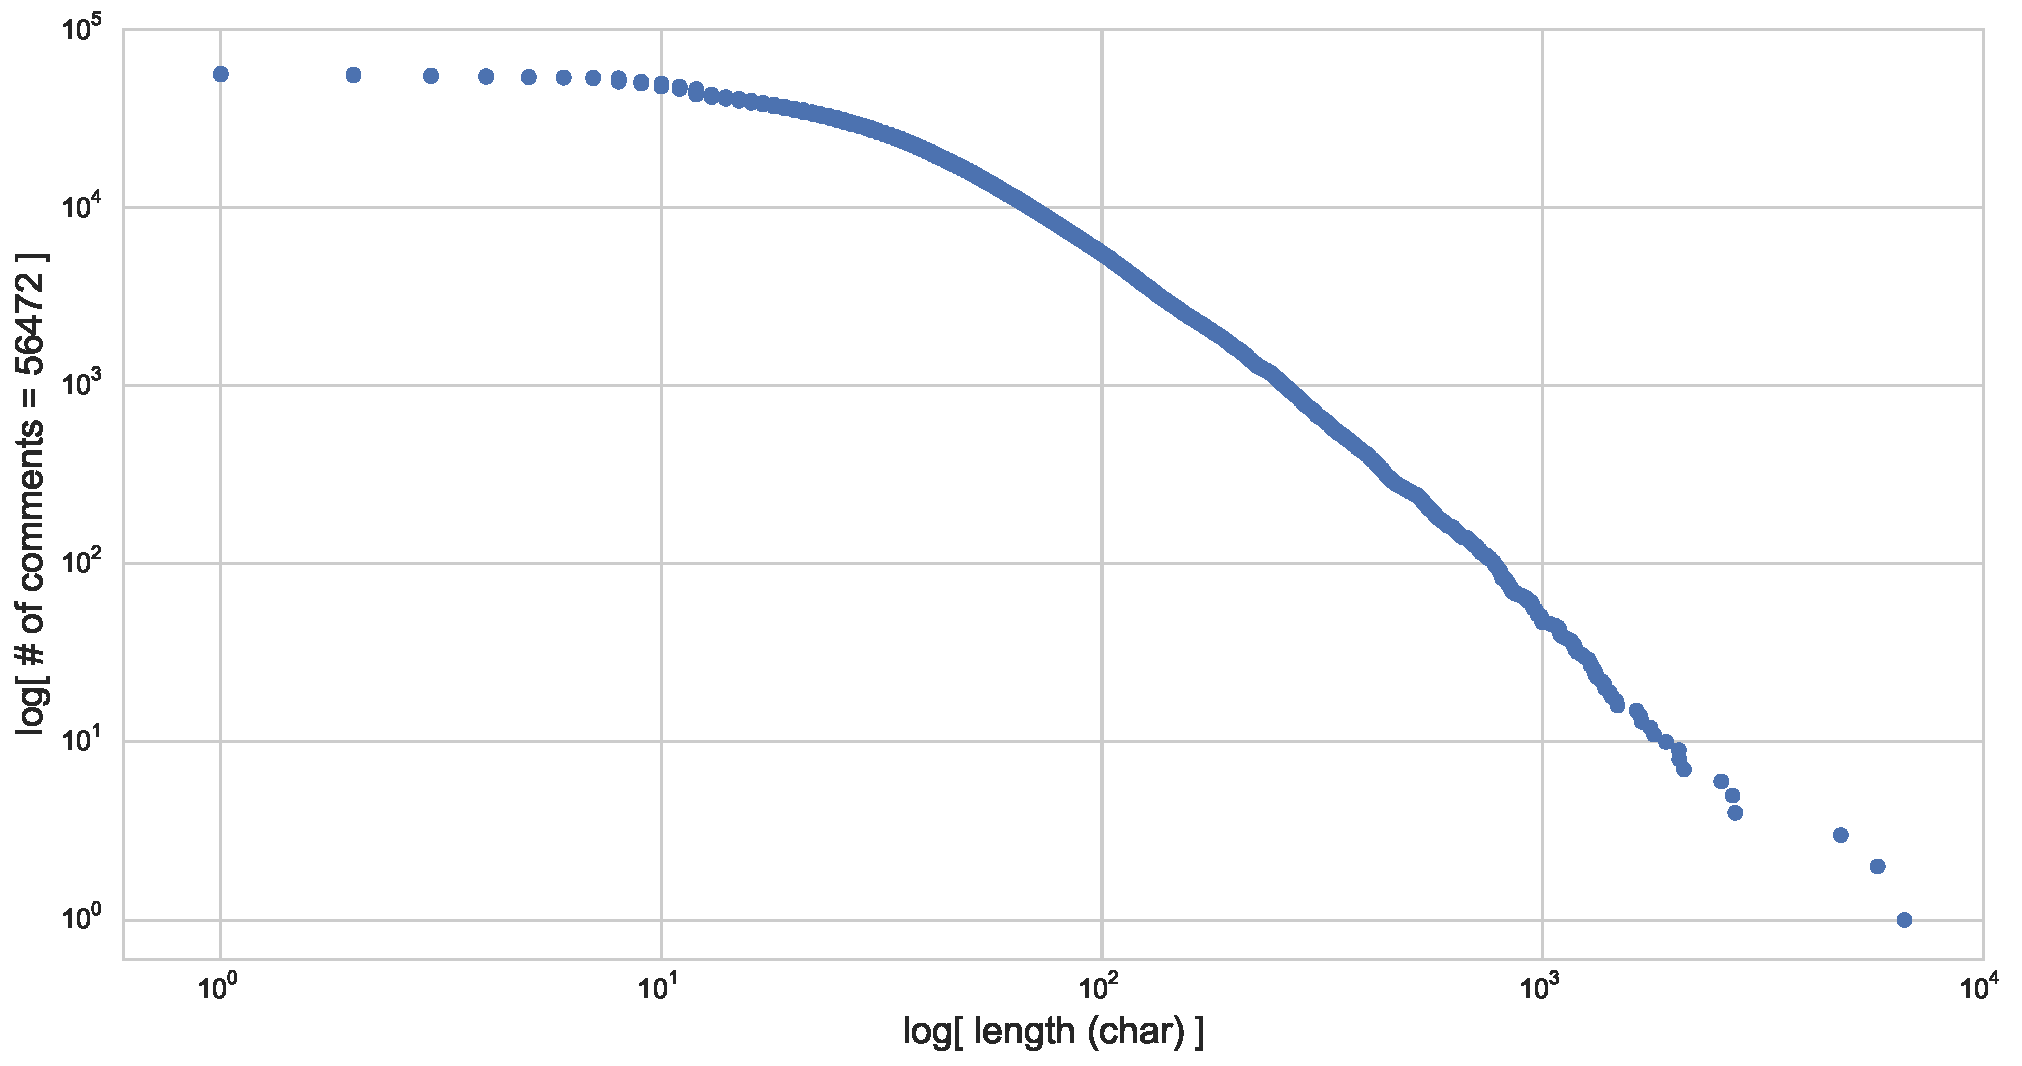
\includegraphics[width=.7\linewidth]{figs/CommentsLength.pdf}
  \caption{Comments length.
  \label{fig:CommentsLength}}
\end{figure}

Figure~\ref{fig:CommentsLength} shows the distribution of comments
length, that resembles quite well a power law.

By manually inspecting the comments, it seems clear that some sort of
refinement would be helpful, if not needed.
Table~\ref{tab:refinement} shows some of the refinement that we
executed (automatically, by a script) on every comment. 
Then, the same analyses have been performed on both the raw and
refined comments.

\begin{table}[tp]
  \begin{center}
    \tbl{Some examples of comment refinement: raw form on the
      left, refined form on the right. \^{} represents the start of the
      comment. About 15k comments out of the total about 56k are
      modified by these changes. 
      \label{tab:refinement}
    }{%
      \begin{tabular}{l lcl}
        \toprule
        &Raw form & $\longrightarrow$ & Refined form\\
\midrule
        1. lowercase everything \\
\addlinespace
        2. typos
        &relelevant & $\longrightarrow$ & relevant\\
        &relelevance & $\longrightarrow$ & relevance\\
\addlinespace        
        3. Contractions
        &does not & $\longrightarrow$ & doesn't\\
        &doesnt & $\longrightarrow$ & doesn't\\
\addlinespace
        4. Synonyms
        &notrelevant & $\longrightarrow$ & irrelevant\\
        &nonrelevant & $\longrightarrow$ & irrelevant\\
        &irrelevante & $\longrightarrow$ & irrelevant\\
        &irelevant & $\longrightarrow$ & irrelevant\\
        &es irrelevante & $\longrightarrow$ & it is irrelevant\\
        &not relevant & $\longrightarrow$ & irrelevant\\
        &non relevant & $\longrightarrow$ & irrelevant\\
        &article & $\longrightarrow$ & document\\
\addlinespace        
        5. Semantic conflations
        &\^{}this document & $\longrightarrow$ & the document\\
        &\^{}it's about & $\longrightarrow$ & the document is about\\
        &\^{}it's not about & $\longrightarrow$ & the document is not about\\
        &\^{}not about & $\longrightarrow$ & the document is not about\\
        &\^{}about & $\longrightarrow$ & the document is about\\
        &\^{}it is & $\longrightarrow$ & the document is\\
        &\^{}its about & $\longrightarrow$ & the document is about\\
        &\^{}its not about & $\longrightarrow$ & the document is not about\\
        &\^{}is about & $\longrightarrow$ & the document is about\\
\addlinespace        
        &\^{}it has nothing to do & $\longrightarrow$ & the document has nothing to do\\
        &\^{}this document has nothing to do & $\longrightarrow$ & the document has nothing to do\\
        \bottomrule
      \end{tabular}%
    } 
  \end{center}
\end{table}

We use two comment representations:
\begin{itemize}
\item A vector space based representation: we build a vector space for
  comments and documents using 1,2,3-grams and tf.idf.   
  \fs{Why not just use a simple (unigram) term presence/absence
    vector, or tf.idf vector? 
    Also, need to give tf.idf instantiation?}
  \sm{If I remember it correctly, we started with unigrams and then by
    looking at the comments it seemed more reasonable to use n-grams
    than unigrams, though I do not remember the details now... 
    Eddy, do you remember?
    But you're right that we should look at the results with unigrams
    as well.}
  Then, we measure the similarity among comments with classical cosine
  similarity. 
  We also measure the similarity between comments and documents in the
  same way.
\item A topic models based representation: \sm{...}
\end{itemize}


\subsection{Comment Similarity}
\label{sec:comment-similarity}

We report on several pairwise similarity comparisons. 
We compare (i) the similarity of a comment:
\begin{itemize}
\item on the same topic,
\item on the same document,
\item on  documents having similar relevance (measured as TREC
  relevance, Sormunen relevance, and workers's normalized ME
  scores), and
\item by the same worker (remember that some workers tended to work
  ``in sessions'', see
  end of Section~\ref{sec:crowd-judging}),
\end{itemize}
with (ii)  the similarity of the comment with any other comment.
% We compare: (i) the similarity of a comment with a generic comment
% \fs{(not sure what a generic comment is -- any other comment out of all
% 50,000?)}
% and (ii) the similarity of the comment with comments:
% \begin{itemize}
% \item on the same topic; 
% \item on the same document; 
% \item on
%   documents having similar relevance (measured as TREC
%   relevance, Sormunen relevance, and  workers's normalized ME
%   scores); 
% \item by the same worker (recall and re-discuss ``sessions'', see
%   end of Section~\ref{sec:crowd-judging}).
% \end{itemize}
We also compare (i) the similarity of the comment with ``its'' document,
i.e., the document that was being judged when the comment was
expressed, with (ii) the similarity of a comment with any other document.

The following charts show that there is a clear influence of all these
factors: comments exhibit a higher similarity with comments on the
same topic (Figure~\ref{fig:simIntraExtraTopic}), with comments on the
same document (Figure~\ref{fig:simIntraExtraDocument}), with comments
on documents having similar relevance
(Figure~\ref{fig:simRelevanceLevels}). 
\sm{The boxplot for same
  workers is missing: Eddy can you please do it?} 
Comments also exhibit a higher similarity with the corresponding
document than with the other documents
(Figure~\ref{fig:simItsDocument}).
\fs{I think while the previous figure around topics is interesting we probably don't
need this one as well?}
\sm{These are all placeholders: we need to present a more
  differentiated set, e.g., from refined comments and topic models}

\begin{figure}[tp]
  \centering
  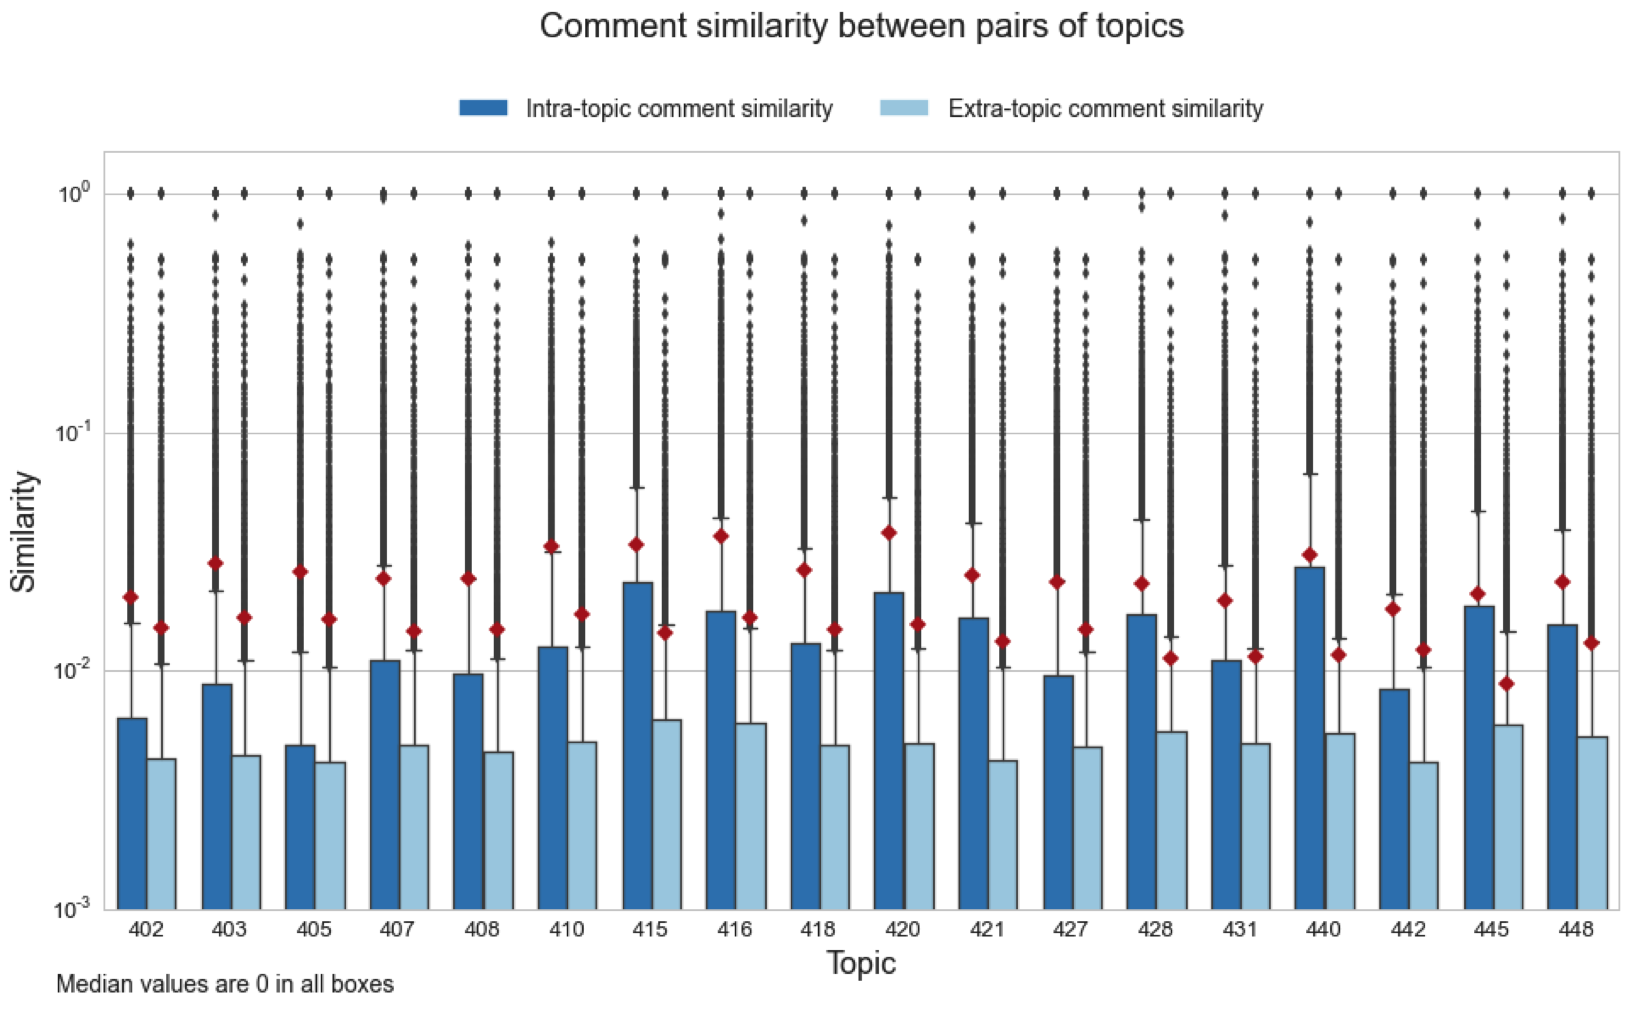
\includegraphics[width=.9\linewidth]{figs/Intra-ExtraTopicSimilarity.png}
  \caption{Similarity of a comment with comments on the same
    topic vs. similarity with comments on other topics.
\fs{Remove title and footnote?}
  \label{fig:simIntraExtraTopic}}
\end{figure}


\begin{figure}[tp]
  \centering
  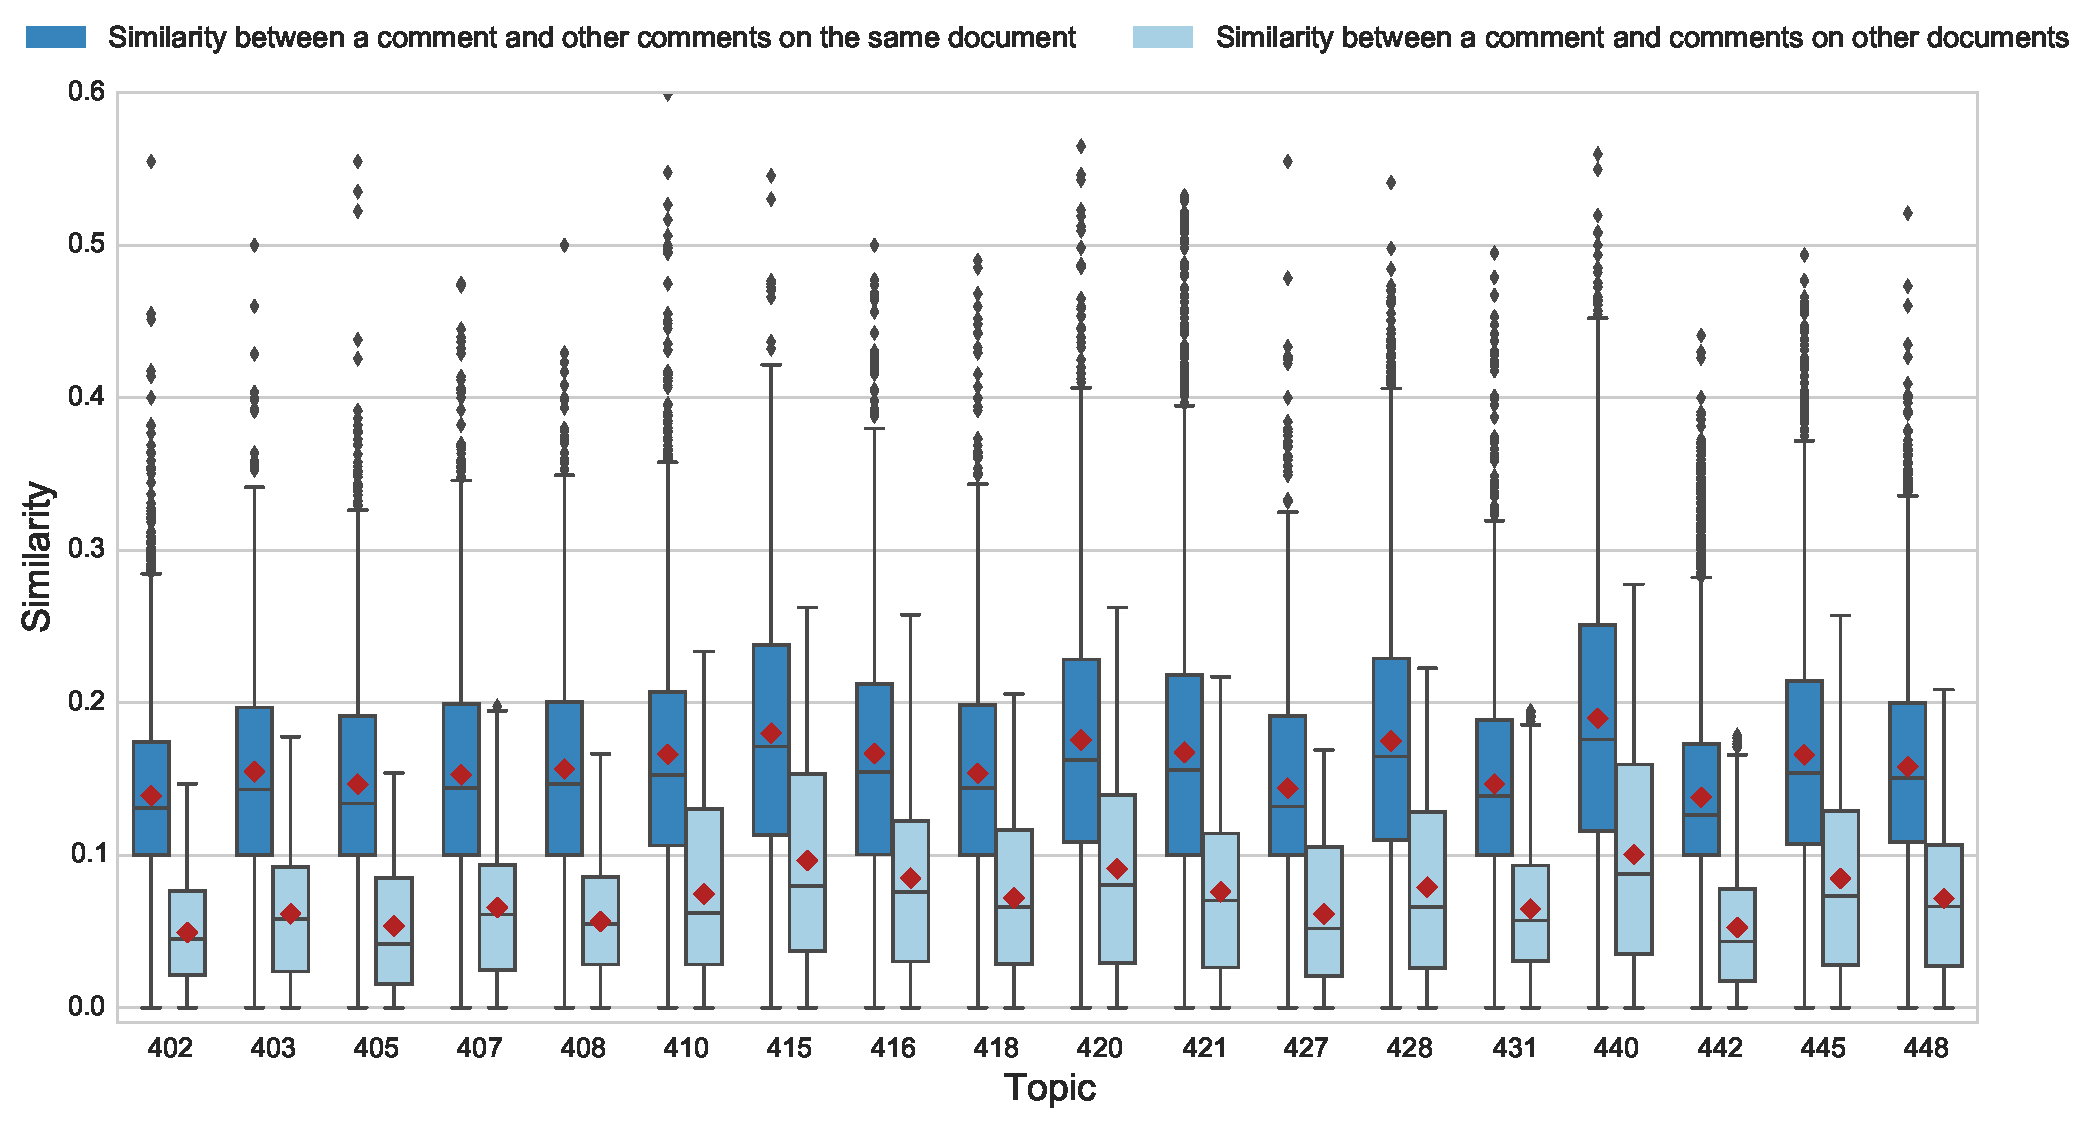
\includegraphics[width=.9\linewidth]{figs/Intra-ExtraDocumentSimilarity.pdf}
  \caption{Similarity of a comment with other comments on the same
    document vs. similarity with comments on other documents.
\fs{Why is this by topic, not by document?}
  \label{fig:simIntraExtraDocument}}
\end{figure}


\begin{figure}[tp]
  \centering
  \begin{tabular}{cc}
  \multicolumn{2}{c}{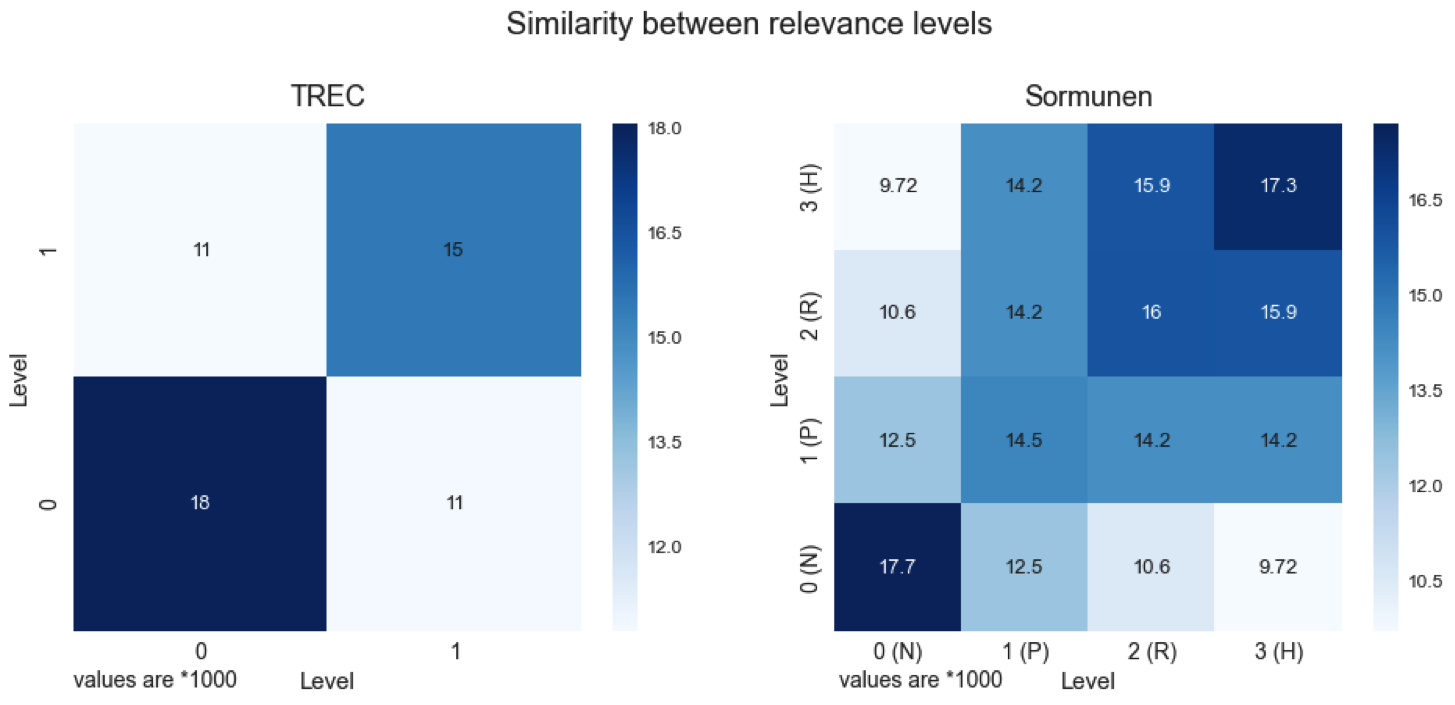
\includegraphics[width=.9\linewidth]{figs/SimilarityTRECSormunen.png}}\\
  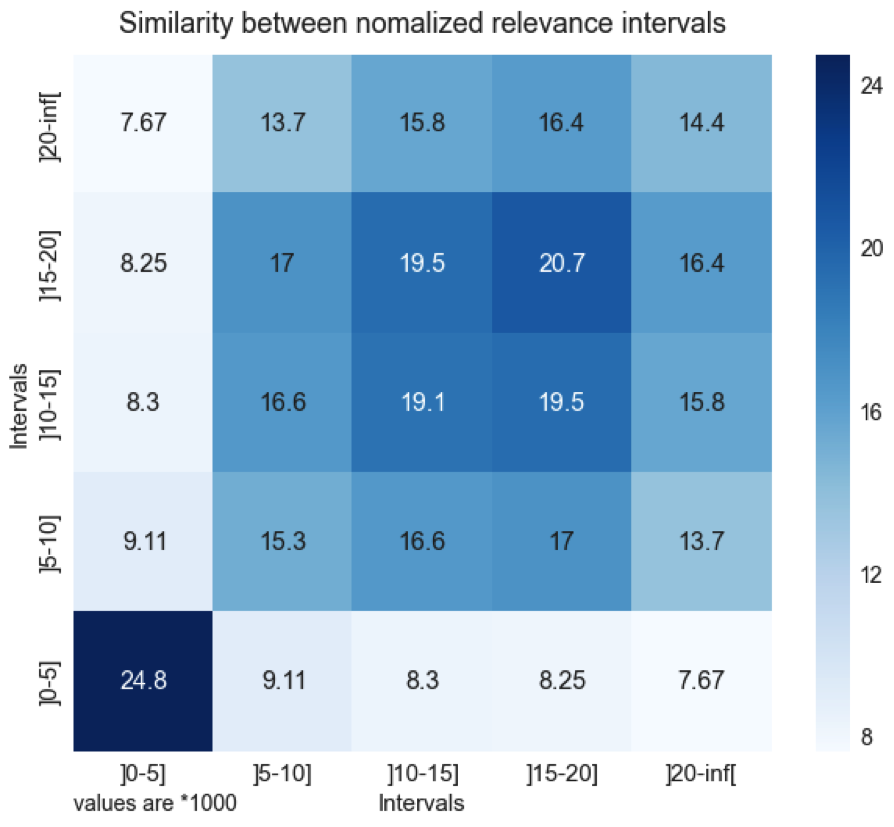
\includegraphics[width=.42\linewidth]{figs/SimilarityIntervals.png}&
  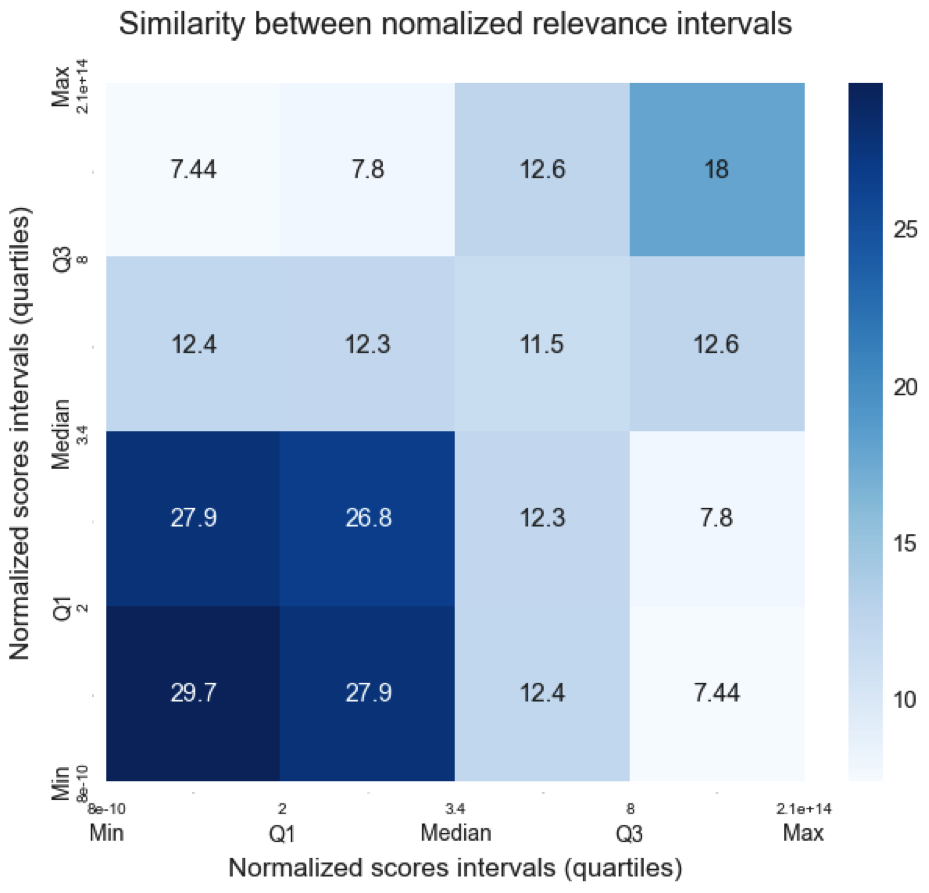
\includegraphics[width=.42\linewidth]{figs/SimilarityQuantiles.png}
  \end{tabular}
  \caption{Similarity of a comment with comments having a particular
    relevance, measured as: TREC relevance (top left), Sormunen
    relevance (top right), and normalized ME scores, divided in equal
    size intervals (bottom left) and quartiles (bottom right). The
    higher values close to the diagonals show that comments are more
    similar when expressed on documents having similar relevance.
  \label{fig:simRelevanceLevels}}
\end{figure}



\begin{figure}[tp]
  \centering
  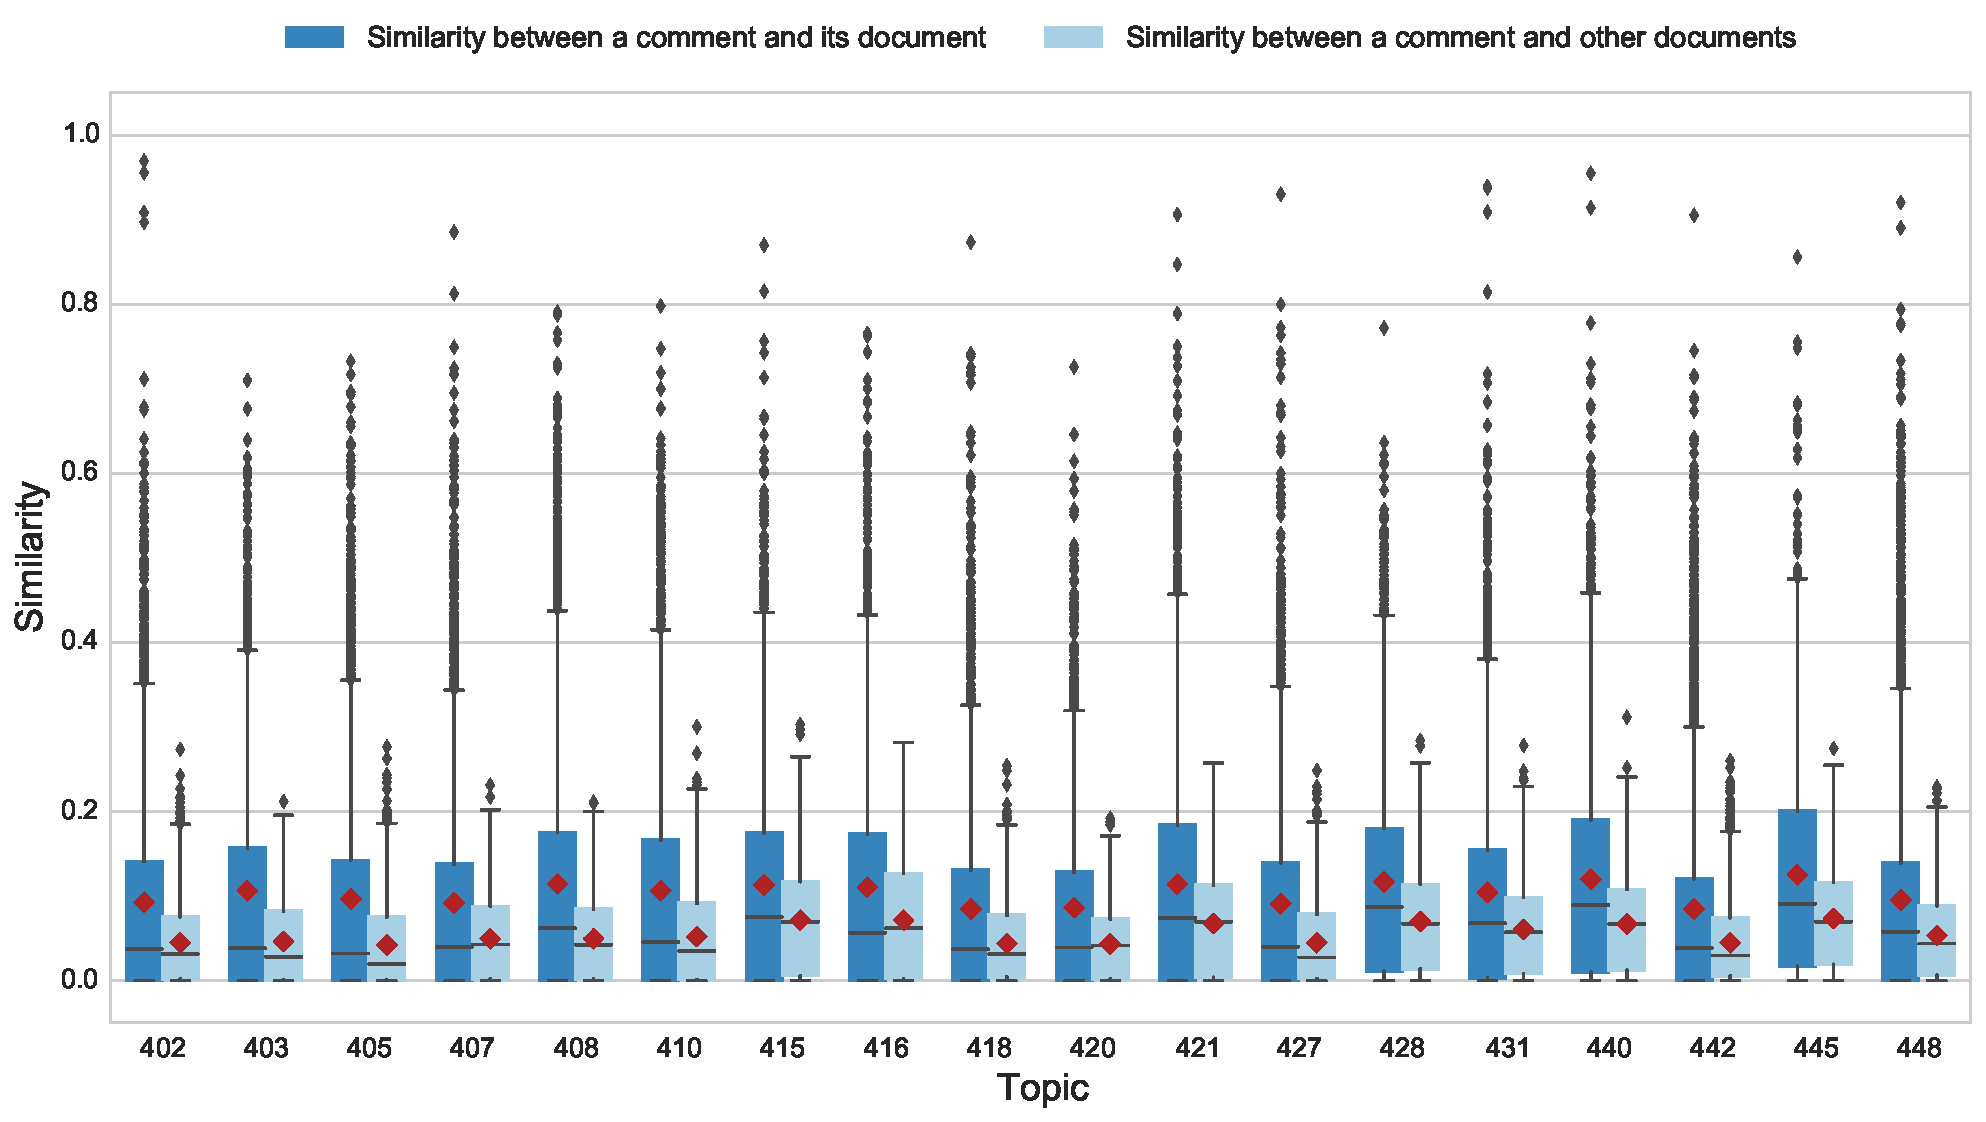
\includegraphics[width=.9\linewidth]{figs/ItsDocumentSimilarity.pdf}
  \caption{Similarity of a comment with its document vs. similarity
    with other documents. 
\fs{Do we need this one?}
  \label{fig:simItsDocument}}
\end{figure}

\sm{add something on Refined Comments}
\sm{add something on topic models}

\subsection{Inductive Coding}
\label{sec:inductive-coding}

\sm{TODO!}
\fs{Pasting in my simplistic first attempt from the google doc below
this comment. If we agree on these categories, we could e.g. sample 200
random comments, and try to categorise them? (And see how well we
agree?)}

\begin{enumerate}
\item statement of relevance or non-relevance -- current document  \\
    "irrelevant"  \\
    "relevant"  \\
    "kinda related"  \\
    "slight relevance"  \\
    "whole document discussing the topic"  \\

\item statement of relevance or non-relevance -- relative  \\
    "the current document not relevant as the previous one"  \\
    "the current document seems as relevant as the previous one"  \\
    "A bit better than previous documents but still irrelevant because it is not talking about poaching in wildlife reserves specifically"  \\

\item comment on topicality or lack of topicality  \\
    "nothing about genetics in this document"  \\
    "deals with cosmic events, but not unexplained or undetected ones"  \\
    "related to drugs and golden triangle but not right location i.e. Iraq  not  Burma, Thailand and Laos"  \\

\item  length of document  \\
    "short"  \\
    "i read part but it ws so long so hopefully i didnt miss anything"  \\

\item direct quote from document  \\
    "The study, directed by Dr. Andrea Z. LaCroix of the Group Health Cooperative of Puget Sound, Wash., was published in the New England Journal of Medicine."  \\

\item junk  \\
    "-"  \\
    " "  \\

\item mixed (e.g. topicality plus statement of relevance/non-relevance)
\fs{Or for mixed, just add them to all categories that they are included in?}

\end{enumerate}





\subsection{Exploiting Comments}
\label{sec:exploiting-comments}

One might think that longer comments correspond to some relevance
level or to higher quality workers. 
We found almost no correlation (around 0.1) between comment length and
the  normalized relevance score. \sm{...}

\sm{Can we infer relevance score from comment text?}

\sm{Can we infer worker quality from comment length? text?}

\subsection{Limits}
\label{sec:limits}


\begin{itemize}
  \item Limit of this study: we left the workers quite free in terms of what kind of
    comment was requested. 
    If this on the one side has the merit of allowing us to gather a
    large variety of comments, it also limited the quality of
    comments.
    We plan to run a follow-up experiment with more precise
    instructions, and to repeat the analysis presented in this section
    on the new dataset. 
    But the methodology presented here should be valid and useful in general.
\end{itemize}

% Local Variables:
% TeX-master: "ME-TOIS.tex"
% End:
